\documentclass[notes,xcolor=dvipsnames]{beamer}
\usepackage{etex}
\usepackage{pgf}
\usepackage{color}
\definecolor{lblue}{rgb}{0.5,0.5,1}
\usepackage{xspace}
\usepackage{listings}
\usepackage{adjustbox}
\usepackage{spverbatim}
\usepackage{subcaption}
\captionsetup{compatibility=false}
\usepackage{textpos}
\usepackage{etoolbox}
\usepackage{xparse}
\usepackage[shadow , roundedcorners, customcolors, getthemecolors]{dynblocks}

\usepackage{tikz}
\usepackage{tikz-qtree}
\usetikzlibrary{shapes,arrows,positioning,shadows,trees,shadows.blur}
\usepackage{pgfplots}
\usepackage{filecontents}
\usepackage{rotating}
\usepackage{graphicx}
\usepackage[round]{natbib}

\mode<presentation>
{
	%\setbeamertemplate{footline}[page number]
	\setbeamertemplate{footline}{%
  \raisebox{2pt}{\makebox[\paperwidth]{\hfill\makebox[20pt]{\textcolor{gray}{\insertframenumber/\inserttotalframenumber}}}}}
  \usetheme{Goettingen}
	%\usecolortheme{dove}
  \setbeamercovered{transparent}
}


\usepackage[english]{babel}
% or whatever

\usepackage[latin1]{inputenc}
% or whatever

\usepackage{times}
\usepackage[T1]{fontenc}
% Or whatever. Note that the encoding and the font should match. If T1
% does not look nice, try deleting the line with the fontenc.

\newcommand{\parspace}{}
%\newcommand{\parspace}{\vspace{-\baselineskip}}
\newcommand{\NN}{\mathbb{N}}
\newcommand{\PP}{\mathbb{P}}
\newcommand{\ZZ}{\mathbb{Z}}
\newcommand{\FF}{\mathbb{F}}           %% for finite fields
\newcommand{\GG}{\mathbb{G}}

\newcommand{\Zrq}{\mathbb{Z}^\ast_q}
\newcommand{\ZN}{\mathbb{Z}_N}

\newcommand{\cA}{\ensuremath{\mathcal{A}}\xspace}
\newcommand{\cB}{\ensuremath{\mathcal{B}}\xspace}
\newcommand{\cC}{\mathcal{C}}
\newcommand{\cD}{\mathcal{D}}
\newcommand{\cE}{\mathcal{E}}
\newcommand{\cF}{\mathcal{F}}
\newcommand{\cG}{\mathcal{G}}
\newcommand{\cH}{\mathcal{H}}
\newcommand{\cI}{\mathcal{I}}
\newcommand{\cK}{\mathcal{K}}
\newcommand{\cL}{\mathcal{L}}
\newcommand{\cM}{\mathcal{M}}
\newcommand{\cO}{\mathcal{O}}
\newcommand{\cP}{\mathcal{P}}
\newcommand{\cQ}{\mathcal{Q}}
\newcommand{\cR}{\mathcal{R}}
\newcommand{\cS}{\mathcal{S}}
\newcommand{\cT}{\mathcal{T}}
\newcommand{\cU}{\mathcal{U}}
\newcommand{\cX}{\mathcal{X}}

\newcommand{\secpar}{\lambda{}}

% assigment, random-choice, etc.
\newcommand{\asgn}{:=}          % assigment \sigma := (a,b,c)
\newcommand{\algout}{\gets}     % algorithm output (sk,pk) <-- KGen(...), hash- and pr-functions too
\newcommand{\ralgout}{\stackrel{R}{\gets}}     % output of random algorithm
\newcommand{\cmp}{=}            % comparison a = b
\newcommand{\rch}{\in_R}        % random choice x \in_R {0,1}^m

\newcommand{\bits}{\{0,1\}}
\newcommand{\rin}{\in_R}
\newcommand{\rinb}{\rin\bits}
\newcommand{\concat}{\!\parallel\!}
%\newcommand{\bitlength}[1]{\lvert{#1}\rvert_{_2}}

\DeclareMathOperator{\ord}{ord}
\DeclareMathOperator{\mymod}{mod}
\newcommand{\MYMOD}[1]{\;(\mymod {#1})}
\DeclareMathOperator{\lcm}{lcm}
\DeclareMathOperator{\dom}{dom}
\newcommand{\legen}[2]{\bigl(\tfrac{#1}{#2}\bigr)}
\newcommand{\jacob}[2]{\bigl(\tfrac{#1}{#2}\bigr)}

\newcommand{\writtenby}[1]{~\mbox{\normalsize\normalfont{(#1)}}}

% new commands
\newcommand{\pwd}{\mathrm{pw}}
\newcommand{\pwdv}{\ensuremath{\mathbf{pw}}}
\newcommand{\msg}{\mathrm{m}}
\newcommand{\mout}{m_{\mathrm{out}}}
\renewcommand{\min}{m_{\mathrm{in}}}
\newcommand{\pake}{\mathrm{PAKE}}
\newcommand{\iencode}{\ensuremath{\mathtt{iEncode}}\xspace}
\newcommand{\idecode}{\ensuremath{\mathtt{iDecode}}\xspace}
\newcommand{\ihme}{\mathrm{IHME}}
\newcommand{\IHME}{\mathtt{IHME}}
\newcommand{\map}{\mathtt{map}}
\newcommand{\mapinv}{\mathtt{mapinv}}
\newcommand{\para}{\mathtt{par}}
\newcommand{\client}{\ensuremath{\mathtt{client}}\xspace}
\newcommand{\server}{\ensuremath{\mathtt{server}}\xspace}
\newcommand{\role}{\mathtt{role}}
\newcommand{\pk}{\ensuremath{\mathtt{pk}}\xspace}
\newcommand{\sk}{\ensuremath{\mathtt{sk}}\xspace}
\newcommand{\Label}{\ensuremath{\mathtt{label}}\xspace}

\newcommand{\comp}{\ensuremath{\mathcal{C}}\xspace}
\newcommand{\round}{\ensuremath{\mathcal{R}}\xspace}
\newcommand{\com}{\ensuremath{\mathcal{E}}\xspace}

\newcommand{\FKV}{$\mathcal{O}$'KV\xspace}
\newcommand{\FBKV}{$\mathcal{O}$'BKV\xspace}
\newcommand{\FSPAKE}{\ensuremath{\mathcal{O}\mathrm{'SPAKE}}\xspace}
\newcommand{\FGMR}{\ensuremath{\mathcal{O}\mathrm{'GMR}}\xspace}

%\newcommand{\mpake}{\mathbb{F}\textnormal{-}\mathrm{PAKE}}
\newcommand{\mpake}{{\ensuremath{\text{O-PAKE}}}\xspace}
\newcommand{\mpakei}{\mathtt{O\text{-}PAKE}}
\newcommand{\D}{\mathcal{D}}
\newcommand{\pgen}{\ensuremath{\mathtt{PGen}}\xspace}
\newcommand{\init}{\ensuremath{\mathtt{init}}\xspace}
\newcommand{\nextm}{\ensuremath{\mathtt{next}}\xspace}
\newcommand{\conf}{\ensuremath{\mathtt{confirm}}\xspace}
\newcommand{\checks}{\ensuremath{\mathtt{check}}\xspace}
\newcommand{\m}{\mathbf{m}}

\newcommand{\sid}{\mathtt{sid}}
\newcommand{\sids}{\pmb{\mathtt{sid}}}
\newcommand{\trans}{\mathtt{trans}}
\newcommand{\NULL}{\mathtt{null}}
\newcommand{\pid}{\mathtt{pid}}
\newcommand{\key}{\ensuremath{\mathtt{k}}\xspace}
\newcommand{\keys}{\ensuremath{\pmb{\mathtt{k}}}\xspace}
\newcommand{\acc}{\mathtt{acc}}
\newcommand{\term}{\mathtt{term}}
\newcommand{\state}{\ensuremath{\mathtt{state}}}
\newcommand{\states}{\pmb{\mathtt{state}}}
\newcommand{\used}{\mathtt{used}}
\newcommand{\send}{\ensuremath{\mathsf{Send}}\xspace}
\newcommand{\execute}{\ensuremath{\mathsf{Execute}}\xspace}
\newcommand{\reveal}{\ensuremath{\mathsf{Reveal}}\xspace}
\newcommand{\test}{\ensuremath{\mathsf{Test}}\xspace}
\newcommand{\corrupt}{\ensuremath{\mathsf{Corrupt}}\xspace}
\newcommand{\create}{\ensuremath{\mathtt{Create}}\xspace}
\newcommand{\INIT}{\ensuremath{\mathsf{Init}}\xspace}

\newcommand{\MYIF}{\mathtt{If}}
\newcommand{\MYELSE}{\mathtt{Else}}
\newcommand{\MYTHEN}{\mathsf{Then}}

\newcommand{\advo}{\cA_1(\secpar)}
\newcommand{\advt}{\cA_2(\secpar)}

\newcommand{\true}{\mathtt{true}}
\newcommand{\Adv}{\mathsf{Adv}}
\newcommand{\Succ}{\mathsf{Succ}}
\newcommand{\prob}{\ensuremath{\mathrm{Pr}}\xspace}
\newcommand{\Exp}{\ensuremath{\mathsf{Exp}}\xspace}
\newcommand{\Expi}[1]{\ensuremath{\mathsf{Exp}_{#1}}\xspace}
\newcommand{\Expbm}[1]{\ensuremath{\bm{\mathsf{Exp}_{#1}}}\xspace}
\newcommand{\ake}{\mathsf{AKE\text{-}Sec}}
\newcommand{\AKE}{\mathsf{AKE}}
\newcommand{\ROR}{\mathrm{ROR}}
\newcommand{\FTG}{\mathrm{FTG}}
\newcommand{\cauth}{\mathsf{CAuth}}
\newcommand{\sauth}{\mathsf{SAuth}}
\newcommand{\pwhide}{\mathsf{PW\text{-}Hid}}
\newcommand{\npwhide}{n\mathsf{\text{-}PW\text{-}Hid}}
\newcommand{\akefull}{\mathsf{AKE\text{-}FSec}}
\newcommand{\akecpa}{\mathsf{AKE\text{-}CPWA}}
\newcommand{\simul}{\mathsf{Sim}}
\newcommand{\Sim}{\ensuremath{\mathsf{Sim}}\xspace}
\newcommand{\ext}{\mathsf{Ext}}
\newcommand{\calls}{\textnormal{ calls }}
\newcommand{\refalgo}[2]{Algorithm \ref{#1}, Line \ref{#2}}
\newcommand{\refline}[1]{Line \ref{#1}}
\newcommand{\ihide}{\mathsf{ihide}}
\newcommand{\dlin}{\ensuremath{\mathsf{DLIN}}}
\newcommand{\genbg}{{\ensuremath{\mathsf{GenBG}}}}
\newcommand{\cca}{\ensuremath{\mathsf{CCA}}\xspace}
\newcommand{\St}{\mathtt{St}}

\newcommand{\KDF}{\ensuremath{\mathtt{KDF}}\xspace}
\newcommand{\PRF}{\ensuremath{\mathrm{PRF}}\xspace}
\newcommand{\prf}{\ensuremath{\mathtt{prf}}\xspace}
\newcommand{\Enc}{\ensuremath{\mathtt{Enc}}\xspace}
\newcommand{\Dec}{\ensuremath{\mathtt{Dec}}\xspace}
\newcommand{\Gen}{\ensuremath{\mathtt{Gen}}\xspace}
\newcommand{\Mac}{\ensuremath{\mathtt{MAC}}\xspace}

\newcommand{\tbf}[1]{\\\textbf{#1}}

\newcommand{\myhref}[2]{\href{#1}{#2}\footnote{\url{#1}}}

\newcommand{\naive}{na{\"i}ve\xspace}

\newcommand{\myparagraph}[1]{\paragraph{#1.}}
\newcommand{\mysubsubsection}[1]{\subsubsection{#1.}}

\newcommand{\TabEQ}{%
       \setlength{\abovedisplayskip}{-\topskip}%
       \setlength{\belowdisplayskip}{-\topskip}%
}

\newlength{\arrow}
\settowidth{\arrow}{\scriptsize$10000000000000000$}
\newcommand*{\myrightarrow}[1]{\xrightarrow{\mathmakebox[\arrow]{#1}}}
\newcommand*{\myleftarrow}[1]{\xleftarrow{\mathmakebox[\arrow]{#1}}}
\newcommand*{\myleftrightarrow}[1]{\xleftrightarrow{\mathmakebox[\arrow]{#1}}}

\newlength{\shortarrow}
\settowidth{\shortarrow}{\scriptsize$1000000$}
\newcommand*{\myshortrightarrow}[1]{\xrightarrow{\mathmakebox[\shortarrow]{#1}}}
\newcommand*{\myshortleftarrow}[1]{\xleftarrow{\mathmakebox[\shortarrow]{#1}}}
\newcommand*{\myshortleftrightarrow}[1]{\xleftrightarrow{\mathmakebox[\shortarrow]{#1}}}

\newcommand{\marked}[2]{{\color{red}}#2}

\title[Password Based Authentication] % (optional, use only with long paper titles)
{Advancments in Password Based Authentication}

\author[F. Kiefer] % (optional, use only with lots of authors)
{Franziskus Kiefer}
% - Give the names in the same order as the appear in the paper.
% - Use the \inst{?} command only if the authors have different
%   affiliation.

\institute[University of Surrey] % (optional, but mostly needed)
{
 Department of Computing Science\\
 University of Surrey
}
% - Use the \inst command only if there are several affiliations.
% - Keep it simple, no one is interested in your street address.

\date[Viva] % (optional, should be abbreviation of conference name)
{PhD Viva}
% - Either use conference name or its abbreviation.
% - Not really informative to the audience, more for people (including
%   yourself) who are reading the slides online

\subject{Password Based Authenticated Key Exchange, PAKE}
% This is only inserted into the PDF information catalog. Can be left
% out. 



% If you have a file called "university-logo-filename.xxx", where xxx
% is a graphic format that can be processed by latex or pdflatex,
% resp., then you can add a logo as follows:

\pgfdeclareimage[height=0.5cm]{university-logo}{University-of-Surrey-logo.jpg}
\logo{\pgfuseimage{university-logo}}



% Delete this, if you do not want the table of contents to pop up at
% the beginning of each subsection:
%\AtBeginSubsection[]
%{
%  \begin{frame}<beamer>{Outline}
%    \tableofcontents[currentsection,currentsubsection]
%  \end{frame}
%}


% If you wish to uncover everything in a step-wise fashion, uncomment
% the following command: 

%\beamerdefaultoverlayspecification{<+->}


\begin{document}

 \tikzset{
    %Define standard arrow tip
    >=stealth',
    %Define style for boxes
    party/.style={
           rectangle,
           rounded corners,
           draw=black, very thick,
           text width=6.5em,
           minimum height=2em,
           text centered},
    state/.style={
           inner sep=0,
           minimum size=0cm},
    box/.style={draw=none,shade,
      top color=blue!40,
      bottom color=blue!5,
      rounded corners=6pt,
      blur shadow={shadow blur steps=5},
      text width=6em},
    bigbox/.style={draw=none,shade,
      top color=blue!40,
      bottom color=blue!5,
      rounded corners=6pt,
      blur shadow={shadow blur steps=5},
      text width=2em,
      minimum height=12em},
    % Define arrow style
    pil/.style={
           ->,
           thick,
           shorten <=2pt,
           shorten >=2pt,},
    circle dotted/.style={dash pattern=on .05mm off 2mm, line cap=round}
}

\begin{frame}
  \titlepage
\end{frame}

\begin{frame}{Outline}
  \tableofcontents %[pausesections]
  % You might wish to add the option [pausesections]
\end{frame}


\section{Introduction \& Motivation}

\subsection{Authentication and Key Exchange}

\begin{frame}{How to Communicate Securely? (1/2)}

	How can I communicate securely with a website?
	
	\pause
	\vspace*{2em}
	\setbeamercolor{uppercol}{fg=white,bg=blue}%
	\setbeamercolor{lowercol}{fg=black,bg=lblue}%
	\begin{beamerboxesrounded}[upper=uppercol,lower=lowercol,shadow=true]{\centering TLS}\centering
		TLS and HTTPS 
	\end{beamerboxesrounded}

  \pause
	\vspace*{2em}
  How to securely communicate individualised content from a website?

	\pause
	\vspace*{2em}
	\setbeamercolor{uppercol}{fg=white,bg=blue}%
	\setbeamercolor{lowercol}{fg=black,bg=lblue}%
	\begin{beamerboxesrounded}[upper=uppercol,lower=lowercol,shadow=true]{\centering Passwords}\centering
		Password over HTML
	\end{beamerboxesrounded}
\end{frame}
	
\begin{frame}{How to Communicate Securely? (2/2)}

	How can two (or more) parties want to communicate securely?
	
	\vspace*{2em}
	\structure{Secure}
	\begin{itemize}
		\item Authentic
		\item Confidential
	\end{itemize}

	\vspace*{2em}
	\structure{Key-Establishement} rather than expensive asymmetric encryption
	\begin{itemize}
		\item Key Transport/Distribution
		\item<1-| alert@2> Key Exchange/Agreement
	\end{itemize}
\end{frame}
	
\begin{frame}{Authenticated Key Exchange}

\begin{figure}
\centering
\begin{tikzpicture}
	\node[state,align=center] (client) at (0,0.25) {\pgfimage[width=0.8cm]{os_tux}\\\alert{s}};
	
	\node[state, align=left] (clientText) at (0,-1) {accept $k$};
	\node[state] (client1) at (2,-1){};
	
	\node[state, align=left] at (0,-2) {};
	\node[state] (client2) at (2,-2){};	
	
	
	\node[state,align=center] (server) at (6,0.25) {\pgfimage[width=0.8cm]{techie_sailor}\\\alert{s}};
	
	\node[state, align=right] (serverText) at (6,-1) {accept $k$};
	\node[state] (server1) at (4,-1) {};
	
	\node[state, align=right] at (6,-2) {};
	\node[state] (server2) at (4,-2) {};
	
	\node[cylinder, blue, draw,minimum height=1.5cm, minimum width=1.5cm,aspect=.5, inner xsep=1.5cm, inner ysep=0.5cm] at (2.9,-2) {};
	\draw[pil,<->] (client1) -- node[above] {Key Exchange} (server1);
	\draw[pil,<->] (server2) -- node[above] {Secure Channel} (client2);
	
	\draw[pil,->] (clientText.west) |- (1.5,-2);
	\draw[pil,->] (serverText.east) |- (4.5,-2);
\end{tikzpicture}
%\caption{Encrypted Key Exchange (EKE)}
\label{fig:ke}
\end{figure}

\structure{Authenticated} Key Exchange
\begin{itemize}
	\item Requires \alert{(common) secret}
\end{itemize}

\end{frame}

\subsection{Password Authenticated Key Exchange}

\begin{frame}{Password Authenticated Key Exchange}{PAKE 1/2}
	\begin{quote}
	``Humans are incapable of securely storing high-quality cryptographic keys, and they have unacceptable speed and accuracy when performing cryptographic operations.''~\cite{Kaufmann02}
	\end{quote}
	
	\pause
	\vspace*{2em}
	\setbeamercolor{uppercol}{fg=white,bg=blue}%
	\setbeamercolor{lowercol}{fg=black,bg=lblue}%
	\begin{beamerboxesrounded}[upper=uppercol,lower=lowercol,shadow=true]{\centering Passwords}\centering
		Common secret with low entropy
	\end{beamerboxesrounded}
	
\end{frame}

\begin{frame}{Password Authenticated Key Exchange}{PAKE 2/2}
	Inherent threat of dictionary attacks
	\begin{itemize}
		\item Can not prevent online dicionary attacks
		\item PAKE Security:\\\begin{center} \alert{security against offline dictionary attacks}\end{center}
	\end{itemize}
	
	\vspace*{2em}
	Established security models
	\begin{itemize}
		\item Game Based Security Model by \cite{Bellare2000}%[BPR 2001]
		\item Universally Composable PAKE by \cite{Canetti2005}%[CHKLK 2005]
	\end{itemize}
%	Well established research area since 2000
%	\begin{itemize}
%		\item Simple password-based encrypted key exchange protocols by \cite{Abdalla2005}
%		\item Faster and shorter password-authenticated key exchange by \cite{Gennaro2008}
%		\item Round-Optimal Password-Based Authenticated Key Exchange by \cite{Katz2011}
%		\item \dots
%	\end{itemize}
\end{frame}

\begin{frame}{Password Authenticated Key Exchange}{SPAKE}

 \cite{Abdalla2005}: SPAKE uses DL-hard group $G$ and public $M,N\in G$; hash function $H$ as random oracle

\begin{figure}
\centering
\begin{tikzpicture}
	\node[state] (client) at (0,0.25) {\pgfimage[width=0.8cm]{os_tux}};
	
	\node[state, align=left] at (0,-1) {$x\rin\ZZ_p, X\gets g^x$\\  $\color{red} X'\gets X\cdot M^\pwd$};
	\node[state] (client1) at (2,-1){};
	
	\node[state, align=left] at (0,-2) {$K'_A\gets {\color{red} (Y'/N^\pwd)}^x$};
	\node[state] (client2) at (2,-2){};	
	
	%\node[state, align=center] at (0,-3) {$K\gets H(A,B,X',Y',K_A,\pwd)$};
	
	
	\node[state] (server) at (6,0.25) {\pgfimage[width=0.8cm]{techie_sailor}};
	
	\node[state, align=right] at (6,-1) {$y\rin\ZZ_p, Y\gets g^y$\\ $\color{red} Y\gets Y\cdot N^\pwd$};
	\node[state] (server1) at (4,-1) {};
	
	\node[state, align=right] at (6,-2) {$K'_B\gets {\color{red} (X'/M^\pwd)}^y$};
	\node[state] (server2) at (4,-2) {};
	
	%\node[state, align=center] at (6,-3) {$K\gets H(A,B,X',Y',K_B,\pwd)$};
	
	\draw[pil] (client1) -- node[above] {$X'$} (server1);
	\draw[pil] (server2) -- node[above] {$Y'$} (client2);
\end{tikzpicture}
\label{fig:eke}
\end{figure}
Key derivation:\\
$K_A\gets H(A,B,X',Y',K'_A,\pwd)$\\
$K_B\gets H(A,B,X',Y',K'_B,\pwd)$

\end{frame}

\subsection{PAKE Security Models}

\begin{frame}{PAKE Security Model 1/2}{Authenticated Key Exchange (AKE) 1/2}
The PPT adversary $\mathcal{A}$ has access to the following oracles:
\begin{description}
    \item[$m'\gets\mathsf{Send}(P,P',m)$:] \hfill \\ simulates active attack.
    \item[$\mathtt{t}\gets\mathsf{Execute}(P,P')$:] \hfill \\ simulates passive attack
    \item[$\pwd\gets\mathsf{Corrupt}(P, P')$:] \hfill \\ simulates password leakage
    \item[$\mathtt{k}_\mathcal{A}\gets\mathsf{Test}(P)$:] \hfill \\ returns real or random key (security definition)
\end{description}
\end{frame}

\begin{frame}{PAKE Security Model 1/2}{Authenticated Key Exchange (AKE) 2/2}
\begin{definition}[AKE-Security]\label{def:ake}
A PAKE protocol $\Pi$ is \emph{AKE-secure} if for all dictionaries $\mathcal{D}$ and for all PPT adversaries $\mathcal{A}$ using at most $t$ active attacks there exists a negligible function $\varepsilon(\cdot)$ such that:
\[\left|\Pr[\mathsf{Exp}_{\Pi,\mathcal{A}}^{\mathsf{AKE-SEC}}(\varepsilon)=1]-\frac12\right|\leq \frac{\mathcal{O}(t)}{|\mathcal{D}|}+\varepsilon(\lambda).\]

\noindent$\mathsf{Exp}_{\Pi,\mathcal{A}}^{\mathsf{AKE-SEC}}(\lambda):$ \\
\hspace*{2em} $b\in_R\{0,1\}$\\
\hspace*{2em} $b'\gets\mathcal{A}^{\mathsf{Send},\mathsf{Execute},\mathsf{Corrupt},\mathsf{Test}}(\lambda)$\\
\hspace*{2em} return $b=b'$
\end{definition}
$\mathsf{Test}$ may only be asked on \emph{fresh} session.
\end{frame}

\begin{frame}{PAKE Security Model 2/2}{Universal Composability (UC) 1/2}
The following entities are involved:
\begin{description}
    \item[$\mathcal{Z}$:] \hfill \\ environmnet/distinguisher
    \item[$\Pi$:] \hfill \\ a real-world PAKE protocol
    \item[$\mathcal{A}$:] \hfill \\ real-world adversary on $\Pi$
    \item[$\mathcal{F}_{\text{PAKE}}$:] \hfill \\ ideal funcitonality for PAKE protocols
    \item[$\mathcal{S}$:] \hfill \\ ideal-world adversary
\end{description}
\end{frame}

\begin{frame}{PAKE Security Model 2/2}{Universal Composability (UC) 2/2}
\begin{definition}[UC-Security]\label{def:uc}
A PAKE protocol $\Pi$ is \emph{UC-secure} if distinguisher $\mathcal{Z}$ is not able to decide whether it is interacting with the real world protocol $\Pi$ and the real world adversary $\mathcal{A}$ or the ideal functionality $\mathcal{F}$ and ideal-world adversary $\mathcal{S}$.
\end{definition}

\end{frame}

% \begin{frame}{Forward-Secrecy in PAKE 1/4}{}
%
% 	Forward-Secrecy is modelled with corruptions
% 	\begin{itemize}
% 		\item Forward-Secrecy: session key will not be compromised if long-term key is compromised in the future
% 		\item Corrupt oracle returns long-term secret (password)
% 	\end{itemize}
%
% \end{frame}
%
% \begin{frame}{Forward-Secrecy in PAKE 2/4}{Corruption Models}
%
% 	\begin{description}
% 		\item[Zero] \hfill \\ $\mathcal{A}$ has no access to the $\mathsf{Corrupt}$ oracle.
% 		\item[Static] \hfill \\ $\mathcal{A}$ has no access to the $\mathsf{Corrupt}$ oracle but can initially retrieve passwords before the experiment starts.
% 		\item[Adaptive] \hfill \\ $\mathcal{A}$ has access to the $\mathsf{Corrupt}(C,S)$ oracle to retrieve $\pwd_{(C,S)}$.
% 		\item[Strong] \hfill \\  $\mathcal{A}$ has access to the $\mathsf{Corrupt}(C,S)$ oracle to retrieve state information of all client instances $C_i$ that have been invoked with server $S$, including $\pwd_{C,S}$.
% 	\end{description}
%
% \end{frame}
%
% \begin{frame}{Forward-Secrecy in PAKE 3/4}{}
%
% 	\begin{dynblock}
% 		First block
% 		\opaqueblock<1>{
% 				\begin{quote}
% 					``The set of malicious users did not need to be considered in the 2-party due to the independence among the passwords shared between pairs of honest participants and those shared with malicious users.''
% 				\end{quote}
% 				\vskip5mm
% 			  \hspace*\fill{\small--- \cite{Abdalla2005a}}
% 		}
% 		\invblock<2->
%
% 		Second block
% 		\opaqueblock<2>{
% 				\begin{quote}
% 					``In the password-only setting, this [static corruption] actually makes no difference because the adversary can internally simulate these oracles by itself.''
% 				\end{quote}
% 				\vskip5mm
% 			  \hspace*\fill{\small--- \cite{Gennaro2008}}
% 		}
% 		\invblock<3->
%
% 		Third block
% 		\opaqueblock<3>{
% 				\begin{quote}
% 					``[...] we consider the original BPR2000 model without [dynamic] Corrupt query because the basic notion of BPR2000 freshness restricts the adversary [...] from corrupting anyone in the model (i.e., effectively restricting $\mathcal{A}$ from asking any Corrupt query).''
% 				\end{quote}
% 				\vskip5mm
% 			  \hspace*\fill{\small--- \cite{ChooBH05}}
% 		}
% 	\end{dynblock}
%
% \end{frame}
%
% \begin{frame}{Forward-Secrecy in PAKE 4/4}{}
%
% 	However
% 	\begin{itemize}
% 		\item No proof for equality of static/adaptive and zero corruption model given
% 		\item No counterexample in the two-party setting exists
% 	\end{itemize}
% 	
% 	\vspace*{2em}
% 	\structure{Contribution}
% 	\begin{itemize}
% 		\item Consolidation of corruption models
% 		\item Impossibility of secure PAKE in the strong corruption model
% 		\item Unfortunately, no proof for equality of adaptive and zero corruption model found (yet)
% 	\end{itemize}
%
% \end{frame}

%===============================================================================
% A Password Authentication Framework for the Single-Server Setting
%===============================================================================

\section{Single-Server Password Framework}%{A Password Authentication Framework for the Single-Server Setting}

\begin{frame}{Table of Content}
\tableofcontents[currentsection]
\end{frame}

\newsavebox{\savelisting}
\newenvironment{listing}
{\vspace*{-2em}\begin{lrbox}{\savelisting}
\begin{minipage}{4.8in}
\begin{flushleft}}
{\end{flushleft}
\end{minipage}
\end{lrbox}
\begin{center}
\resizebox{\columnwidth}{!}{\setlength\fboxsep{6pt}\fbox{\usebox{\savelisting}}}
\end{center}}

\subsection{Modelling Password Policies}

\subsection[ZKPPC]{Zero-Knowledge Password Policy Checks}

\subsection[BPR]{Blind Password Registration}

\subsection[SPC]{Secure Set-based Policy Checking}

\subsection[VPAKE]{Verifier-based PAKE}

% \begin{frame}[fragile]{Password Based Authentication on the Web}{}
%
% \renewcommand{\figurename}{}
% \begin{figure}
% 	\centering
% 	\caption{TLS Channel}
% 	
\includegraphics[width=.6\textwidth]{loginForm2.png}
% \end{figure}
%
% \begin{figure}
% \centering
% \caption{HTML Form}
% \begin{subfigure}[t]{0.5\textwidth}
% 	\centering
% 	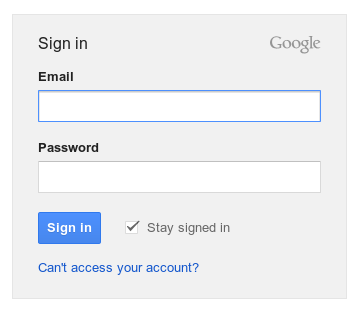
\includegraphics[width=\textwidth]{loginForm.png}
% \end{subfigure}%
% ~
% \begin{subfigure}[t]{0.5\textwidth}
% \centering
% \vspace*{-9.75em}
% \begin{listing}
% \begin{spverbatim}
% <h2>Sign in <strong></strong></h2>
% <form novalidate id="gaia_loginform" action="https://accounts.google.com/ServiceLoginAuth" method="post">
%
%
% <div class="email-div">
%   <label for="Email"><strong class="email-label"> Username</strong></label>
%   <input type="email" spellcheck="false" name="Email" id="Email" value="">
% </div>
%   
% <div class="passwd-div">
%   <label for="Passwd"><strong class="passwd-label"> Password</strong></label>
%   <input type="password" name="Passwd" id="Passwd">
% </div>
% <input type="submit" class="g-button g-button-submit" name="signIn" id="signIn" value="Sign in">
% \end{spverbatim}
% \end{listing}
% \end{subfigure}
%
% \end{figure}
%
% \end{frame}
%
% %\begin{frame}{Password Based Authentication on the Web}{Drawbacks}
% %	\begin{itemize}
% %		\item Requires \structure{PKI}
% %		\item Server receives \structure{passwords in clear}
% %		\item User has to \structure{remember} passwords \& password-username-server mapping
% %	\end{itemize}
% %	\pause 
% %	\vspace*{2em}	
% %	
% %	\setbeamercolor{uppercol}{fg=white,bg=blue}%
% %	\setbeamercolor{lowercol}{fg=black,bg=lblue}%
% %	\begin{beamerboxesrounded}[upper=uppercol,lower=lowercol,shadow=true]{\centering }\centering
% %		...Not the best way to do it...
% %	\end{beamerboxesrounded}
% %	
% %	\pause 
% %	\vspace*{2em}	
% %	
% %	\setbeamercolor{uppercol}{fg=white,bg=blue}%
% %	\setbeamercolor{lowercol}{fg=black,bg=lblue}%
% %	\begin{beamerboxesrounded}[upper=uppercol,lower=lowercol,shadow=true]{\centering Better Solution}\centering
% %		Password Based Authenticated Key Exchange
% %	\end{beamerboxesrounded}
% %	
% %\end{frame}
%
% \begin{frame}{PAKE on the Web}{}
%
% 	\begin{figure}
% \centering
% \begin{tikzpicture}
% 	\node[state, align=left] at (-0.5,-2) {\pgfimage[width=2cm]{browser}};
% 		
% 	\node[state] (client1) at (1.5,-1){};
% 	\node[state] (client4) at (1.5,-2.5){};
% 	
% 	\node[state, align=right] at (7.5,-2) {\pgfimage[width=2cm]{web_server}};
%
% 	\node[state] (server1) at (4.75,-1) {};
% 	\node[state] (server4) at (4.75,-2.5) {};
% 	
% 	\draw[pil,<->] (client1) -- node[above] {\texttt{PAKE}} (server1);
%
% 	\node[state, align=left] at (3,-1.5) {\structure{Secured$_K$}};	
% 	\node[cylinder, blue, draw,minimum height=1.5cm, minimum width=1.5cm,aspect=.5, inner xsep=2cm, inner ysep=0.5cm] at (3,-2.5) {};
% 	\draw[pil,<->] (client4) -- node[above] {} (server4);
% \end{tikzpicture}
%
% \end{figure}
%
% \vspace*{1em}
%
% 	\begin{itemize}
% 		\item No server certificates (PKI) needed
% 		\item Passwords are \structure{not transmitted} at all
% 	\end{itemize}	
%
% \vspace*{1em}
%
% 	\structure{However}, PAKE protocols are \structure{hardly used} in practice (missing standards / incompatibility may be a reason)
%
% \end{frame}
%
% \subsection{Oblivious PAKE}
%
% \begin{frame}{The Problem of Failed Logins}{}
%
% 	Users still struggle with passwords (cf. \cite{Florencio2007,Gaw2006a}):
% 	
% 	\begin{itemize}
% 		\item 2.4 failed login attempts on average
% 		\item 6.5 different passwords in use\\ (on approx. 25 accounts)
% 		\item \structure{Password disclosure} with current practice
% 	\end{itemize}
% 	\pause\vspace*{1em}
%
% 	\begin{columns}[t]
%     \begin{column}{.475\linewidth}
% 	    	{\centering\structure{PAKE}}\\
% 	    	\begin{itemize}
% 	    		\setlength{\itemindent}{-1em}
% 	    		\item Run $n$ PAKE protocols
% 		    \item Linear amount of work
% %	    		\item Communication overhead
% 	    	\end{itemize}
%     \end{column}
% 	\vspace*{2em}
%     \begin{column}{.475\linewidth}
%     		{\centering\structure{TLS-based}}\\
%     		\begin{itemize}
% 	    		\setlength{\itemindent}{-1em}
% 	    		\item Establish 1 TLS channel
% 	    		\item Send $n$ forms
%     		\end{itemize}
%     \end{column}
%   \end{columns}
% %	SPAKE execution for $3$ passwords: $3\times4$ Exponentiations%, $3\times2$ Multiplications, $3$ Inversions, $3$ Hashes
% \end{frame}
%
% \begin{frame}{Oblivious PAKE}{Contribution}
%
% 	\setbeamercolor{uppercol}{fg=white,bg=blue}%
% 	\setbeamercolor{lowercol}{fg=black,bg=lblue}%
% 	\begin{beamerboxesrounded}[upper=uppercol,lower=lowercol,shadow=true]{}\centering
% 		Efficient PAKE with multiple client input passwords
% 	\end{beamerboxesrounded}
%
% 	
% 	\pause	
% 	\vspace*{2em}	
% 	
% 	\structure{Goals}	
% 	
% 	\begin{itemize}
% 		\item \structure{Efficient} handling of password trials
% 		\item \structure{No leakage} of non-matching passwords to the server
% 		\item Ease user's password handling
% 	\end{itemize}
% 	
% \end{frame}
%
% \subsection{Setting}
%
% \begin{frame}{Oblivious PAKE}{Setting}
%
% 	\begin{itemize}
% 		\item Client and server share password $\pwd$
% 		\item Client inputs a list of up to $c$ passwords $\pwdv$
% 		\item Server can restrict $c$ due to online dictionary attacks
% 	\end{itemize}
%
% \centering\structure{Successful iff $\pwd\in\pwdv$}	
% \begin{figure}
% \centering
% \begin{tikzpicture}
% 	\node[state] (client) at (0,0.5) [align=center]{\pgfimage[width=0.8cm]{os_tux}\\ Client};
% 	
% 	\node[state, align=left] at (0,-1) {$\pwdv$,  $|\pwdv|\leq c$};
% 	\node[state] (client1) at (1.2,-1){};
% 	\node[state] (client2) at (1.2,-2){};
% 	
% 	\node[state] (server) at (6,0.5) [align=center]{\pgfimage[width=0.8cm]{techie_sailor}\\ Server};
% 	
% 	\node[state, align=center] at (6,-1) {$\pwd$};
% 	\node[state] (server1) at (5.6,-1) {};
% 	\node[state] (server2) at (5.6,-2) {};
% 	
% 	\node[state] (middle1) at (3.7,-1.2) {};
% 	\node[state] (middle2) at (3.7,-1.0) {};
%
% 	\node[box] (box) at (3.2,-1)[align=center]{\large O-PAKE};
% 	
% 	\draw[pil] (client1) -- (box);
% 	\draw[pil] (server1) -- (box);
% 	
% 	\draw[pil] ($(box.south)-(0.7,0)$) |- node[below] {\hspace*{-2em}$k_C$}(client2);
% 	\draw[pil] ($(box.south)-(-0.7,0)$) |- node[below] {\hspace*{3em}$k_S$}(server2);
% 	
% 	%\draw[pil,<->] (client1) -- node[above] {$\mathrm{PAKE}_{\pwd}$} (server1);
% 	%\draw[pil] (middle2) edge [loop above, ->,out=70,in=320,distance=1cm] (middle1);
% 	
% \end{tikzpicture}
% %\caption{Encrypted Key Exchange (EKE)}
% %\label{fig:eke}
% \end{figure}		
% 	
% \end{frame}
%
% %\begin{frame}{Oblivious PAKE}{Setting}
% %\begin{figure}
% %	
\includegraphics[width=\textwidth]{loginForm2.png} %FIXME
% %\end{figure}
% %\end{frame}
%
% %\begin{frame}{Oblivious PAKE}{Security Model}
% %	Game based security model from \cite{Bellare2000,Abdalla2005a}: %[BPR 2001, AFP 2005]:
% %	\begin{itemize}
% %		\item Real-or-Random (multiple Test queries)
% %		\item Forward Secrecy (Corrupt oracle)
% %		\item Extended to allow multiple input passwords
% %	\end{itemize}
% %	
% %	\begin{figure}
% %		\fbox{
% %		\begin{tikzpicture}
% %			\node[state, align=left] at (3,-1) {$c\in\NN, b\rin\bits$\\
% %				$\forall(P,P')\in\cC\times\cS$, pick $\pwd_{P,P'}\rin\cD$\\
% %				$b'\gets\cA^{\send,\execute,\corrupt,\test}(\secpar, c)$\\
% %				return $b\cmp b'$};
% %		\end{tikzpicture}}
% %	\end{figure}
%
% %\end{frame}
%
% \begin{frame}{Oblivious PAKE}{Na{\"i}ve Solution}
%
% \setblockcolor{blue!10}
% \setbordercolor{blue!15}
%
% \begin{dynblock}
% % First block
% \opaqueblock<1>{\vspace*{-1em}
% \begin{figure}
% \centering
% \includegraphics[width=\textwidth]{npake.pdf}
% \end{figure}
% }
% \invblock<2->
%
% % Second block
% \opaqueblock<2>[0.6\textwidth]{
% Run $c$ sessions of the same PAKE
% 	\begin{itemize}
% 		\item \structure{Client:}\\\hspace*{2em}
% 		linear amount of work
% 		\item \structure{Server:}\\\hspace*{2em}
% 		linear amount of work
% 	\end{itemize}
% \vspace*{1em}
% Successful iff 1 session successful
% }
%
% \end{dynblock}
%
% \end{frame}
%
% % ------------------------------
% \newcommand{\drawoverlays}{%
% \node[rectangle,draw=black,rounded corners, fill=black!20, text width=5.25em, minimum height=12em] (client) at (2.95,-2.5){}; %draw=black, very thick,
% \node[rectangle,draw=black,rounded corners, fill=black!20, text width=5.25em, minimum height=12em] (client) at (6.2,-2.5){};
% \node[rectangle,draw=black,rounded corners, fill=black!20, text width=26em, minimum height=2.2em] (client) at (3,-7.1){};
% }
%
% \newcommand{\drawoverlay}{%
% \node[rectangle,draw=black,rounded corners, fill=black!20, text width=26em, minimum height=2.2em] (client) at (3,-7.1){};
% }
%
% \newcommand{\drawopake}[6]{%
% \begin{frame}{Oblivious PAKE}{#5}
% \begin{figure}
% \vspace*{-1em}
% \centering
% \scalebox{0.8}{%
% \begin{tikzpicture}%,text width=0em
% 	\node[state] at (1,1.2) [align=center]{\pgfimage[width=0.8cm]{os_tux}\\ Client};	
% %
% 	\node[state, align=left] at (-1.5,-1) {$\mathbf{pw}[1]$};
% 	\node[state, align=left] at (-1.5,-4) {$\mathbf{pw}[c]$};
% 	\node[state] (client1) at (-1,-1){};
% 	\node[state] (client2) at (-1,-2.5){};
% 	\node[state] (client25) at (-1,-4){};
% 	\node[state] (client3) at (-1,-4.5){};
% %	
% 	\node[state] at (6.5,1.2) [align=center]{\pgfimage[width=0.8cm]{techie_sailor}\\ Server};
% %	
% 	\node[state, align=right] at (8.2,-1) {pw};
% 	\node[state] (server1) at (8.1,-2.5) {};
% 	\node[state] (server2) at (8,-1) {};
% 	\node[state] (server25) at (8.4,-4) {};
% 	\node[state] (server3) at (8.4,-4.5) {};
% %	
% 	\node[box, text width=3.5em] (box1) at (.5,-1)[align=center]{\large PAKE};
% 	\node[box, text width=3.5em] (box2) at (.5,-4)[align=center]{\large PAKE};
% %	
% 	\node[bigbox, text width=1.5em] (box3) at (2.25,-2.5)[align=center]{\large #1};
% 	\node[bigbox, text width=1.5em] (box4) at (3.65,-2.5)[align=center]{\large #2};
% 	\node[bigbox, text width=1.5em] (box5) at (5.5,-2.5)[align=center]{\large #3};
% 	\node[bigbox, text width=1.5em] (box52) at (6.9,-2.5)[align=center]{\large #4};
% %	
% 	\node[box, text width=3.5em] (box6) at (7.3,-5.75)[align=center]{\large PAKE};
% %	
% 	\draw[pil] (box1.east) -- node[above] {$m_1$}(box1-|box3.west);
% 	\draw[pil] (box2.east) -- node[above] {$m_c$}(box2-|box3.west);
% 	\draw[pil] ([yshift=1.5cm]box3.east) -- ([yshift=1.5cm]box4.west);
% 	\draw[pil] ([yshift=-1.5cm]box3.east) -- ([yshift=-1.5cm]box4.west);
% 	\draw[pil] (box4.east) -- (box4-|box5.west);
% 	\draw[pil] (box5.east) -- (box5-|box52.west);
% %	
% 	\draw[line width = .5mm,circle dotted] ($(client1)-(0.5,0.5)$) -- ($(client2)-(0.5,1)$);
% 	\draw[line width = .5mm,circle dotted] ($(box1)-(0,0.5)$) -- ($(box2)-(0,-0.5)$);
% %	
% 	\draw[pil] (client1) -- (box1);
% 	\draw[pil] (client25) -- (box2);
% 	\draw[pil] (server2) -- (server2-|box5.east); % -- +(0,.7)
% 	\draw[pil] (box52.east) -| node[right]{$m$}($(box6.north)+(0.5,0)$);
% 	\draw[pil] ($(server2)+(0.5,0.1)$) |- (box6.east);
% %	
% 	\node[rectangle,draw=black,rounded corners, draw=black, very thick, text width=17em, minimum height=20em] (client) at (1,-3.75){};
% 	\node[rectangle,draw=black,rounded corners, draw=black, very thick, text width=9.6em, minimum height=20em] (server) at (6.7,-3.75){};
% 	\node[rectangle,draw=black,rounded corners, draw=black, very thick, text width=16em, minimum height=13em] (clientpake) at (1.05,-2.5){};
% %	
% 	\draw[pil] (box6.west) -| node[below] {$m$}(clientpake.south);
% %
% 	\node[box, text width=6.5em] (box7) at (6.5,-7)[align=center]{\large Confirmation};
% 	\node[box, text width=8em] (box8) at (0,-7)[align=center]{\large Key Derivation};
% %
% 	\draw[pil] (box6.south) -- node[auto] {$k$}(box6|-box7.north);
% 	\draw[pil] (box7) -- node[auto] {$k_f$}($(box7)-(0,1.2)$);
% 	\draw[pil] ([xshift=-1cm]clientpake.south) -- node[left] {$(k_1,\dots,k_c)$}([xshift=-1cm]clientpake|-box8.north);
% 	\draw[pil] (box7.west) -- node[auto] {conf}(box8.east);
% 	\draw[pil] (box8) -- node[auto] {$k_f$}($(box8)-(0,1.2)$);
% % Gray overlays %
% 	#6
% \end{tikzpicture}}
% \end{figure}
% \end{frame}
% }
%
% %\subsection{Idea}
%
% \drawopake{?}{?}{?}{?}{Idea}{\drawoverlays}
%
%
% \subsection{Building Blocks}
%
% \begin{frame}{Building Blocks}{Index-Hiding Message Encoding (IHME)}
%
% 	IHME, introduced by \cite{Manulis2010}, is a message encoding with following properties: %[MPP 2010]
% 	%\vspace*{1em}
% 	\begin{itemize}
% 		\item Encodes set of index, message pairs $(i,m)$
% 		\item Ensures hiding of index $i$
% 		\item Length preserving
% 	\end{itemize}
%
% 	\vspace*{1em}
%
% 	\setbeamercolor{uppercol}{fg=white,bg=blue!40}%
% 	\setbeamercolor{lowercol}{fg=black,bg=blue!20}%
% 	\pause
% 	\begin{beamerboxesrounded}[upper=uppercol,lower=lowercol,shadow=true]{$S\gets\iencode(P)$}
% 		$P=\{(\pwdv[1],m_{1}),\dots,(\pwdv[c],m_{c})\}\rightarrow S=(a_{c-1},\dots,a_0)$\\\\
% 		$f=\sum^{c-1}_{k=0}a_kx^k$ s.t. $f(\pwdv[i])=m_{i}~~\forall(\pwdv[i],m_{i})\in P$
% 	\end{beamerboxesrounded}
% 	
% 	\vspace*{1em}
%
% 	\begin{beamerboxesrounded}[upper=uppercol,lower=lowercol,shadow=true]{$m\gets\idecode(S, \pwd)$}
% 		$(S=(a_{c-1},\dots,a_0), \pwd)\rightarrow m$ with	$m=f(\pwd)$
% 	\end{beamerboxesrounded}
% 	
% \end{frame}
%
% %\begin{frame}{Building Blocks}{Index-Hiding Message Encoding (IHME)}
% %
% %	\setbeamercolor{uppercol}{fg=white,bg=blue!40}%
% %	\setbeamercolor{lowercol}{fg=black,bg=blue!20}%
% %	\begin{beamerboxesrounded}[upper=uppercol,lower=lowercol,shadow=true]{$S\gets\iencode(P)$}
% %		$P=\{(\pwdv[1],m_{1}),\dots,(\pwdv[c],m_{c})\}\rightarrow S=(a_{c-1},\dots,a_0)$\\\\
% %		$f=\sum^{c-1}_{k=0}a_kx^k$ s.t. $f(\pwdv[i])=m_{i}~~\forall(\pwdv[i],m_{i})\in P$
% %	\end{beamerboxesrounded}
% %	
% %	\vspace*{2em}
% %
% %	\begin{beamerboxesrounded}[upper=uppercol,lower=lowercol,shadow=true]{$m\gets\idecode(S, \pwd)$}
% %		$(S=\sum^{c-1}_{k=0}a_kx^k, \pwd)\rightarrow m$\\\\
% %		$m=f(\pwd)$
% %	\end{beamerboxesrounded}
% %
% %
% %\end{frame}
%
% \drawopake{?}{\begin{sideways}\alert{IHME.iEncode}\end{sideways}}{\begin{sideways}\alert{IHME.iDecode}\end{sideways}}{?}{IHME}{\drawoverlay}
%
% \begin{frame}{Building Blocks}{Admissible Encodings}
% 	Admissible Encodings $F:S\rightarrow R, \cI_F:R\rightarrow S$, introduced by \cite{BonehF01} encodes elements from set $S$ to $R$ such that: %[BF 2001, FGKMP 2013] ,BrierCIMRT10,pseudorandomSignatures
% 	\begin{itemize}
% 		\item $\cI_F(r)$ is statistically indistinguishable from uniform distribution over $S$
% 		\item Efficient computable
% 	\end{itemize}
% 	
% 	\pause\vspace*{1em}
% 	%SPAKE uses the following Admissible Encodings to map $G_q\mapsto \ZZ_N$
% 	
% %	\begin{itemize}
% %		\item 
% 		SPAKE uses Admissible Encoding to map arbitrary subgroups $G_q \subseteq \ZZ_N^\ast \mapsto \ZZ_N$ of prime order $q$\\  ~\cite[Lemma~12]{pseudorandomSignatures} %p^\times
% %		\item Set $R=\{0,\dots,N-1\}=\ZZ_N$ of natural numbers, for arbitrary $N\in\NN$. (cf. ~\cite[Lemma~12]{pseudorandomSignatures})
% %	\end{itemize}		
% 	
% \end{frame}
%
% %\begin{frame}{Building Blocks}{Admissible Encodings}
% %Further admissible encodings:
% %\begin{itemize}
% %	\item The set of quadratic residues modulo safe primes~$p$, i.e.\ $R=QR(p)\subseteq\ZZ_p^\times$. (cf. ~\cite[Lemma~12]{pseudorandomSignatures})   
% %    \item The set $R=E(\FF)$ of rational points on (certain) elliptic curves, defined over a finite field (cf. ~\cite{BrierCIMRT10}).
% %\end{itemize}
% %
% %\end{frame}
%
% \drawopake{\begin{sideways}\alert{Admissible Encoding$^{-1}$}\end{sideways}}{\begin{sideways}IHME.iEncode\end{sideways}}{\begin{sideways}IHME.iDecode\end{sideways}}{\begin{sideways}\alert{Admissible Encoding}\end{sideways}}{Admissible Encodings}{\drawoverlay}
%
% \drawopake{\begin{sideways}\alert{Admissible Encoding$^{-1}$}\end{sideways}}{\begin{sideways}IHME.iEncode\end{sideways}}{\begin{sideways}IHME.iDecode\end{sideways}}{\begin{sideways}\alert{Admissible Encoding}\end{sideways}}{Key Confirmation}{}
%
% %\subsection{O-PAKE Compiler}
%
% %\begin{frame}{O-PAKE Compiler}{On the example of SPAKE}
% %	
% %\begin{figure}
% %\centering
% %\resizebox{\textwidth}{!}{%
% %\begin{tikzpicture}
% %	\node[state, align=center, text width=6cm] (client) at (0,1.25) {\pgfimage[width=0.8cm]{os_tux}\\ Client, $\pwdv$};
% %	
% %	\node[state, align=left, text width=6cm] at (0,-1) {\setlength{\baselineskip}{20pt}\alert{For $\pwd_i\in\pwdv$}\\\hspace*{1em} $x\rin\ZZ_p, X\gets g^x$\\\hspace*{1em}  $X'_i\gets X\cdot M^{\pwd_i}$\\\hspace*{1em} \alert{$P=P\bigcup(\pwd_i,\cI_F(X'_i))$} \\ \alert{$S\gets$IHME.encode$(P)$}};
% %	\node[state, text width=6cm] (client1) at (6,-1){};
% %	
% %	\node[state, text width=6cm, align=left] at (0,-5) {\setlength{\baselineskip}{20pt}\alert{For $\pwd_i\in\pwdv$}\\\hspace*{1em} $K'_A\gets (Y'/N^\pwd)^x$\\\hspace*{1em} $K_A^i\gets H(A,B,X',Y',K'_A,\pwd)$\\\hspace*{1em}\alert{$C'\gets\PRF_{K_A^i}(S,Y',0)$}\\\hspace*{1em}\alert{IF $C\cmp C'$}\\\hspace*{2em} \alert{$K_{A_F}\gets\PRF_{K_A}(S,Y',1)$}\\\hspace*{2em}\alert{break}};
% %	\node[state, text width=6cm] (client2) at (0,-3){};
% %	
% %	\node[state, text width=6cm] (client3) at (0,-4.5){};
% %	
% %	%\node[state, align=center] at (0,-3) {$K\gets H(A,B,X',Y',K_A,\pwd)$};
% %	
% %	
% %	\node[state, text width=6cm, align=center] (server) at (6,1.25) {\pgfimage[width=0.8cm]{techie_sailor}\\ Server, $\pwd$};
% %	
% %	\node[state, text width=6cm, align=left] at (7.5,-1) {\setlength{\baselineskip}{20pt}\alert{$X^\ast\gets$IHME.decode$(\pwd,S)$\\ $X'\gets F(X^\ast)$}\\$y\rin\ZZ_p, Y\gets g^y$\\ $Y\gets Y\cdot N^\pwd$};
% %	\node[state, text width=6cm] (server1) at (7,-1) {};
% %	
% %	\node[state, text width=6cm, align=left] at (7.5,-4) {\setlength{\baselineskip}{20pt}$K'_B\gets (X'/M^\pwd)^y$\\ $K_B\gets H(A,B,X',Y',K'_B,\pwd)$\\\alert{$C\gets\PRF_{K_B}(S,Y',0)$}\\\alert{$K_{B_F}\gets\PRF_{K_B}(S,Y',1)$}};
% %	\node[state, text width=6cm] (server2) at (1,-3) {};
% %	
% %	\node[state, text width=6cm] (server3) at (1,-4.5) {};
% %	
% %	%\node[state, align=center] at (6,-3) {$K\gets H(A,B,X',Y',K_B,\pwd)$};
% %	
% %	\draw[pil] (client1) -- node[above] {\alert{$S$}} (server1);
% %	\draw[pil] (server2) -- node[above] {$Y'$} (client2);
% %	\draw[red,pil] (server3) -- node[above] {\alert{$C$}} (client3);
% %\end{tikzpicture}}
% %\end{figure}
%
% %\end{frame}
%
% %\subsection{Implementation \& Performance}
%
% %\begin{frame}{OPAKE Implementation}{}
% %	\structure{Modular} implementation
% %	\begin{itemize}
% %		\item Generic Oblivious PAKE Protocol, including
% %		\begin{itemize}
% %			\item IHME
% %			\item Admissible Encodings for $G_q\mapsto\ZZ_N$
% %		\end{itemize}
% %	\end{itemize}
%
% %	\pause
% %	\vspace*{2em}
% %	Implementing an O-PAKE instance includes:
% %	\begin{itemize}
% %		\item Implementation of suitable PAKE protocols
% %		\item Poss. implementation of an admissible encoding
% %	\end{itemize}
% %	
% %\end{frame}
%
% %\begin{frame}[fragile]{OPAKE Performance}{Oblivious SPAKE Implementation}
% %\begin{figure}[tbp]
% %\centering
% %%	\begin{subfigure}[b]{0.5\textwidth}
% %%		\begin{tikzpicture}[scale=0.85]
% %%		\begin{axis}[xlabel={Number of used Passwords $n$},ylabel={Time [ms]},legend pos= north west,ymax=1200,ymin=0]
% %%			\addplot+[mark=square,black] table[x index=0,y index=6,col sep=space] {measurements.txt};
% %%			\addlegendentry{O-RG-PAKE}		
% %%			\addplot+[mark=triangle,black] table[x index=0,y index=8,col sep=space] {measurements.txt};
% %%			\addlegendentry{N-RG-PAKE}
% %%		\end{axis}
% %%		\end{tikzpicture}
% %%		%\caption{Oblivious RG-PAKE}
% %%		%\label{fig:orgpake}
% %%	\end{subfigure}\hspace*{0.5cm}
% %%	\begin{subfigure}[b]{0.5\textwidth}
% %		\begin{tikzpicture}[scale=0.85]
% %		\begin{axis}[xlabel={Number of used Passwords $n$},ylabel={Time [ms]},legend pos= north west,ymax=50,ymin=0]
% %			\addplot+[mark=square*] table[x index=0,y index=2,col sep=space] {measurements.txt};
% %			\addlegendentry{O-SPAKE}
% %			\addplot+[mark=triangle*] table[x index=0,y index=4,col sep=space] {measurements.txt};
% %			\addlegendentry{N-SPAKE}
% %		\end{axis}
% %		\end{tikzpicture}
% %		%\caption{Oblivious SPAKE}
% %		%\label{fig:ospake}
% %%	\end{subfigure}
% %%	\caption{Server-side Timings for Oblivious RG-PAKE (left) and SPAKE (right) Protocols}\label{fig:orgpake}
% %\end{figure}
% %\end{frame}
%
% \subsection{Summary (Oblivious PAKE)}
%
% \begin{frame}{Summary (Oblivious PAKE)}
%
%   \begin{itemize}
%   \item We proposed \alert{Oblivious PAKE} with multiple client passwords
%   \item \alert{Constant server runtime} even on failed login attempts
%   \item \alert{Modular implementation} of the compiler
%   \item Compiler implementation using SPAKE by \cite{Abdalla2005} and RG-PAKE by \cite{Gennaro2008}
%   \end{itemize}
%   
%   \vskip0pt plus.5fill
%   \begin{itemize}
%   \item
%     Outlook
%     \begin{itemize}
% %    \item Real world application (e.g. browser integration)
%     \item Reduce Communication overhead
%     \item ...
%     \end{itemize}
%   \end{itemize}
% \end{frame}


%===============================================================================
% Password Authentication Framework in the Two-Server Setting
%===============================================================================
\section{2Server Password Framework}%{Password Authentication Framework in the Two-Server Setting}

% \subsection{Distributed Smooth Projective Hashing \& 2-Server PAKE}

\begin{frame}{Table of Content}
\tableofcontents[currentsection]
\end{frame}

\subsection{2Server BPR}

% \subsection{Distributed Smooth Projective Hashing}
\subsection{DSPHF \& A 2-Server PAKE Framework}

\begin{frame}{Smooth Projective Hashing}

\begin{dynblock}
\opaqueblock<1>{\hspace*{1em}
Let $L_x$ denote a language such that $C\in L_x$ if there exists a witness $w$ proving so.
\begin{description}
	\item[$\mathsf{KGen_H}(L_x)$]\hfill\\ generates a hashing key $k_h$ for language $L_x$.
	\item[$\mathsf{KGen_P}(k_h,L_x,C)$]\hfill\\ derives the projection key $k_p$, possibly depending on $C$.
	\item[$\mathsf{Hash}(k_h,L_x,C)$] \hfill\\ outputs the hash value $h$.
	\item[$\mathsf{PHash}(k_p,L_x,C,w)$] \hfill\\ returns the hash value $h$.
\end{description}
}
\invblock<2->

\opaqueblock<2>{\hspace*{1em}
	\begin{description}
		\item[Correctness]\hfill\\ If $C\in L_x$, with $w$ proving so, then $\mathsf{Hash}(k_h,L_x,C)=\mathsf{PHash}(k_p,L_x,C,w)$.
		\item[Smoothness]\hfill\\ If $C\not\in L_x$, the hash value $h$ is statistically indistinguishable from a random element.
		\item[Pseudorandomness]\hfill\\ If $C\in L_x$, the hash value $h$ is indistinguishable from a random element.
	\end{description}
}
\end{dynblock}

\end{frame}

\begin{frame}{PAKE from SPHF}
\begin{figure}
\centering
\begin{tikzpicture}
	\node[state, align=center] (client) at (0,1) {\pgfimage[width=0.8cm]{os_tux}\\ $\pwd$};
	
	\node[state, align=left] at (0,-1) {$k_h\gets\mathsf{KGen_H}(L_x)$\\  $k_p\gets\mathsf{KGen_P}(k_h,L_x)$\\  $C\gets\mathsf{Enc}_\pk(\pwd;r)$};
	\node[state] (client1) at (2,-1){};
	
	\node[state] (client2) at (2,-2){};	
	\node[state, align=left] at (0,-3) {$k\gets\mathsf{Hash}(k_h,L_x,C')$\\$\cdot\mathsf{PHash}(k'_p,L_x,C,r)$};
	
	\node[state, align=center] (server) at (6,1) {\pgfimage[width=0.8cm]{techie_sailor}\\ $\pwd$};
	
	\node[state, align=right] at (6,-1) {$k'_h\gets\mathsf{KGen_H}(L_x)$\\  $k'_p\gets\mathsf{KGen_P}(k_h,L_x)$\\  $C'\gets\mathsf{Enc}_\pk(\pwd;r')$};
	\node[state] (server1) at (4,-1) {};
	
	\node[state] (server2) at (4,-2) {};
	\node[state, align=right] at (6,-3) {$k\gets\mathsf{Hash}(k'_h,L_x,C)$\\$\cdot\mathsf{PHash}(k_p,L_x,C',r')$};
	
	%\node[state, align=center] at (6,-3) {$K\gets H(A,B,X',Y',K_B,\pwd)$};
	
	\draw[pil] (client1) -- node[above] {$C,k_p$} (server1);
	\draw[pil] (server2) -- node[above] {$C',k'_p$} (client2);
\end{tikzpicture}
\label{fig:eke}
\end{figure}
\end{frame}

\begin{frame}{Extended Smooth Projective Hashing 1/2}

%Languages of ciphertexts: $C\gets\mathsf{Enc}_{\pk}(x)$
%2-Server PAKE between \begin{center} Client$(\pwd)$, Server$_1(\pwd_1)$, Server$_2(\pwd_2)$\end{center}

\begin{figure}
\begin{tikzpicture}
	\node[state] (client) at (0,-1) [align=center]{\pgfimage[width=0.8cm]{os_tux}\\ Client $(\pwd)$};
	\node[state] (server1) at (6,0) [align=center]{\pgfimage[width=0.8cm]{techie_sailor}\\ Server 1 $(\pwd_1)$};
	\node[state] (server2) at (6,-2) [align=center]{\pgfimage[width=0.8cm]{techie_sailor}\\ Server 2 $(\pwd_2)$};
	\draw[pil] ($(client.west)+(1.2,0)$) -- (server1);
	\draw[pil] ($(client.west)+(1.2,0)$) -- (server2);
\end{tikzpicture}
\end{figure}

\setbeamercolor{uppercol}{fg=white,bg=blue!40}%
\setbeamercolor{lowercol}{fg=black,bg=blue!20}%
\begin{beamerboxesrounded}[upper=uppercol,lower=lowercol,shadow=true]{\centering Idea}
	Encrypt $\pwd$, $\pwd_1$ and $\pwd_2$ $\rightarrow$ Use extended SPHF to compute keys
\end{beamerboxesrounded}

\end{frame}

\begin{frame}{Extended Smooth Projective Hashing 2/2}

\begin{description}
	\item[$\mathsf{KGen_H}(L_x)$]\hfill\\ generates a hashing key $k_h$ for language $L_x$.
	\item[$\mathsf{KGen_P}(k_h,L_x)$]\hfill\\ derives the projection key $k_h$.
	\item[$\mathsf{Hash}_x (k_{h,0},L_x,C_1,C_2)$]\hfill\\ outputs the hash value $h_x$.
	\item[$\mathsf{PHash}_x (k_{p,0},L_x,C_1,C_2,w_1,w_2)$]\hfill\\ returns the hash value $h_x$.
	\item[$\mathsf{Hash}_0(k_{h,1},k_{h,2},L_x,C_0)$]\hfill\\ outputs the hash value $h_0$.
	\item[$\mathsf{PHash}_0(k_{p,1},k_{p,2},L_x,C_0,w_0)$]\hfill\\ returns the hash value $h_0$.
\end{description}

\end{frame}

\begin{frame}{Distributed (Extended) Smooth Projective Hashing}{DSPHF}

\structure{$\mathsf{PHash}_x^D$} between $S_1$ and $S_2$.\\
	\hspace*{2em} Each $S_i$ performs $\mathsf{PHash}_x^D$ on input $$(k_{p,0},C_1,C_2,w_i)$$\hspace*{2em} such that $S_1$ eventually holds $h_x$.
	
	\vspace*{2em}
\structure{$\mathsf{Hash}_0^D$} between $S_1$ and $S_2$.\\
	\hspace*{2em} Each $S_i$ performs $\mathsf{Hash}_0^D$ on input $$(\pwd_i,k_{h,i}, C_0)$$\hspace*{2em} such that $S_1$ eventually holds $h_0$.

\end{frame}

\begin{frame}{2-Server PAKE from DSPHF}

		\begin{figure}
		\begin{tikzpicture}
			\node[state] (client) at (0,-2) [align=center]{\pgfimage[width=0.8cm]{os_tux}\\ Client $(\pwd)$\\\hspace*{0cm}\\};
			\node[state] (server1) at (6,0) [align=center]{\pgfimage[width=0.8cm]{techie_sailor}\\ Server 1 $(\pwd_1)$};
			\node[state] (server2) at (6,-4) [align=center]{\pgfimage[width=0.8cm]{techie_sailor}\\ Server 2 $(\pwd_2)$};
	
			\draw[pil,->] ($(client.west)+(2,0.2)$) -| node[above,anchor=center,xshift=-1.5cm,yshift=-0.8cm]{$k_p,C$} (server1);
			\draw[pil,->] ($(client.west)+(2,-0.2)$) -| node[below,anchor=center,xshift=-1.5cm,yshift=0.8cm]{$k_p,C$} (server2);
			\draw[pil,<-] ($(client.west)+(1.2,0)$) -- node[above,anchor=center]{$k_{p,1},C_1$} (server1);
			\draw[pil,<-] ($(client.west)+(1.2,0)$) -- node[below,anchor=center]{$k_{p,2},C_2$} (server2);
		\end{tikzpicture}
		\end{figure}

\end{frame}

\begin{frame}{2-Server PAKE from DSPHF}

		\begin{figure}
		\begin{tikzpicture}
			\node[state] (client) at (0,-2) [align=center]{\pgfimage[width=0.8cm]{os_tux}\\ Client $(\pwd)$\\ $\mathsf{PHash}_0\cdot\mathsf{Hash}_x$\\ $\rightarrow \sk$};
			\node[state] (server1) at (6,0) [align=center]{\pgfimage[width=0.8cm]{techie_sailor}\\ Server 1 $(\pwd_1)$\\ $h_x\cdot h_0\rightarrow \sk$};
			\node[state] (server2) at (6,-4) [align=center]{\pgfimage[width=0.8cm]{techie_sailor}\\ Server 2 $(\pwd_2)$};
	
			\draw[pil,<->] (server1) -- node[anchor=center,xshift=-0.1cm]{$\mathsf{PHash}_x^D$~~~~$\mathsf{Hash}_0^D$} (server2);
%			\draw[pil,<-] ($(client.west)+(1.2,0)$) -- node[below,anchor=center]{$k_{p,2},C_2$} (server2);
		\end{tikzpicture}
		\end{figure}

\end{frame}

\subsection{UC 2Server PAKE}

%===============================================================================
% Future Work
%===============================================================================
\section{Summary}

% \begin{frame}{Table of Content}
% \tableofcontents[currentsection]
% \end{frame}

% \subsection{Summary}

\begin{frame}{Summary of Contributions}

\begin{itemize}\itemsep1em
	\item Modelling of Password Policies
	\item Blind Password Registration protocols and model (single and two-server setting)
	\item Distributed SPHF
	\item 2-Server PAKE framework
	\item 2-Server UC PAKE security
\end{itemize}

\end{frame}

% \subsection{Future Work}
%
% \begin{frame}{Future Work}
%
% 	\structure{Work in Progress}
% 	\begin{itemize}
% 		\item Secure Mobile Logins
% 		\item Zero Knowledge Password Policy Checker
% 	\end{itemize}
%
% 	\vspace*{2em}
% 	\structure{Planned Projects}
% 	\begin{itemize}
% 		\item 2-Server PAKE in UC
% 		\item 2-Server password authenticated secret sharing in the password-only model
% 		\item Trying to understand the forward-secrecy in game-based PAKE
% 	\end{itemize}
%
% \end{frame}

%===============================================================================
% Appendix
%===============================================================================

\newcommand{\beginbackup}{
   \newcounter{framenumbervorappendix}
   \setcounter{framenumbervorappendix}{\value{framenumber}}
}
\newcommand{\backupend}{
   \addtocounter{framenumbervorappendix}{-\value{framenumber}}
   \addtocounter{framenumber}{\value{framenumbervorappendix}} 
}

\beginbackup
\appendix
\section<presentation>*{\appendixname}
\subsection<presentation>*{References}

\begin{frame}[allowframebreaks]
  \frametitle<presentation>{References}
  \bibliographystyle{abbrvnat}
  \bibliography{references}
\end{frame}
\backupend

\end{document}
